\chapter{Proyecto}
\section{Introducción}
La capa de Proyecto (Implementación y Despliegue) esta compuesta de los siguientes elementos:

\begin{itemize}
	\item Un paquete de trabajo representa una serie de acciones identificadas y diseñadas para lograr resultados específicos dentro de las limitaciones de tiempo y recursos especificadas.
	\item Un entregable representa un resultado definido con precisión de un paquete de trabajo.
	\item Un evento de implementación es un elemento de comportamiento que denota un cambio de estado relacionado con la implementación o la migración.
	\item Una meseta representa un estado relativamente estable de la arquitectura que existe durante un período de tiempo limitado.
	\item Una brecha representa una declaración de la diferencia entre dos p
\end{itemize}

Una brecha se asocia con los conceptos centrales que son exclusivos de una de las mesetas unidas por la brecha; es decir, los conceptos centrales que constituyen la diferencia entre estas mesetas. Un entregable puede realizar, entre otros, la implementación de una arquitectura o una parte de una arquitectura. Por lo tanto, cualquiera de los conceptos del lenguaje central de ArchiMate puede estar vinculado a un entregable por medio de una relación de realización.\\

Como la mayoría de los conceptos del lenguaje central, un elemento compuesto puede ser un paquete de trabajo agregado o un entregable. También pueden definirse relaciones más débiles. Por ejemplo, la relación de asociación puede utilizarse para mostrar que partes de la arquitectura se ven afectadas de alguna manera por determinados paquetes de trabajo.

%\newpage

\section{Metamodelo}
\begin{figure}[h!]
	\centering
	\includegraphics[width=0.9\linewidth]{imgs/meta/Proyecto}
	\caption{Metamodelo Proyecto}
	\label{fig:mProyecto}
\end{figure}

En la figura \ref{fig:mProyecto} se presenta un panorama general de los elementos de aplicación y migración y sus relaciones.\\

Los elementos de implementación y migración utilizan las relaciones estándar de ArchiMate. Se puede asignar una función comercial a un paquete de trabajo.
Una meseta está ligada a una arquitectura que es válida durante un cierto período de tiempo. Para indicar qué partes de la arquitectura pertenecen a una cierta meseta, una meseta puede agregar o componer cualquiera de los conceptos del lenguaje central de ArchiMate.\\

En sentido estricto, las relaciones entre los elementos de implementación y migración y los elementos de motivación son relaciones indirectas; por ejemplo, un entregable realiza un requerimiento o una meta a través de la realización de un elemento central de ArchiMate (por ejemplo, un componente de aplicación, un proceso de negocios o un servicio). Sin embargo, sigue siendo útil hacer explícitas esas relaciones, para mostrar directamente que un entregable es necesario para realizar ciertos requisitos y objetivos.\\

Además, los objetivos, resultados, capacidades y requisitos pueden asociarse con una cierta meseta; por ejemplo, ciertos requisitos pueden ser sólo aplicables a la Arquitectura de destino, mientras que otros pueden aplicarse a una cierta Arquitectura de transición.\\

Del mismo modo, las mesetas pueden utilizarse para la planificación basada en la capacidad. Esto puede modelarse mediante las relaciones de agregación o composición. Los objetivos, resultados, capacidades y requerimientos pueden ser agregados o compuestos en mesetas. Los requisitos y capacidades pueden realizarse por medio de los resultados. Dado que los resultados y las metas se realizan por medio de las capacidades y los requisitos, también pueden realizarse indirectamente por medio de los productos.

\newpage
\section{Punto de Vista de Proyecto}
\subsection{Modelo de Proyecto}
\begin{figure}[h!]
	\centering
	\includegraphics[width=.9\linewidth]{imgs/modelo/Proyecto}
	\caption{Modelo Proyecto}
\end{figure}
El punto de vista del proyecto se utiliza principalmente para modelar la gestión del cambio de arquitectura del proceso de migración desde una situación antigua (estado actual Enterprise
Arquitectura) a una nueva situación deseada (Arquitectura empresarial del estado de destino) tiene

consecuencias sobre la estrategia de crecimiento a medio y largo plazo y la posterior decisión
proceso de fabricación.  Algunas de las cuestiones que deben tener en cuenta los modelos diseñados en
este mirador son:

Desarrollar una Arquitectura Empresarial completa para toda la organización es una tarea que puede
 requieren varios años.

Todos los sistemas y servicios deben permanecer operativos independientemente del presunto modificaciones y cambios de la Arquitectura Empresarial durante el proceso de cambio.

El proceso de cambio puede tener que lidiar con estándares tecnológicos inmaduros (por ejemplo,
mensajería, seguridad, datos, etc.).

El cambio tiene graves consecuencias para el personal, la cultura, la forma de trabajar y
organización. Además, hay varios otros aspectos de gobernanza que podrían limitar la transformación del proceso, como cooperación interna y externa, gestión de cartera de proyectos, gestión de proyectos (entregables, metas, etc.), planificación de meseta, aspectos financieros y legales, etc.

\subsection{Caso  de Proyecto}
\begin{figure}[h!]
	\centering
	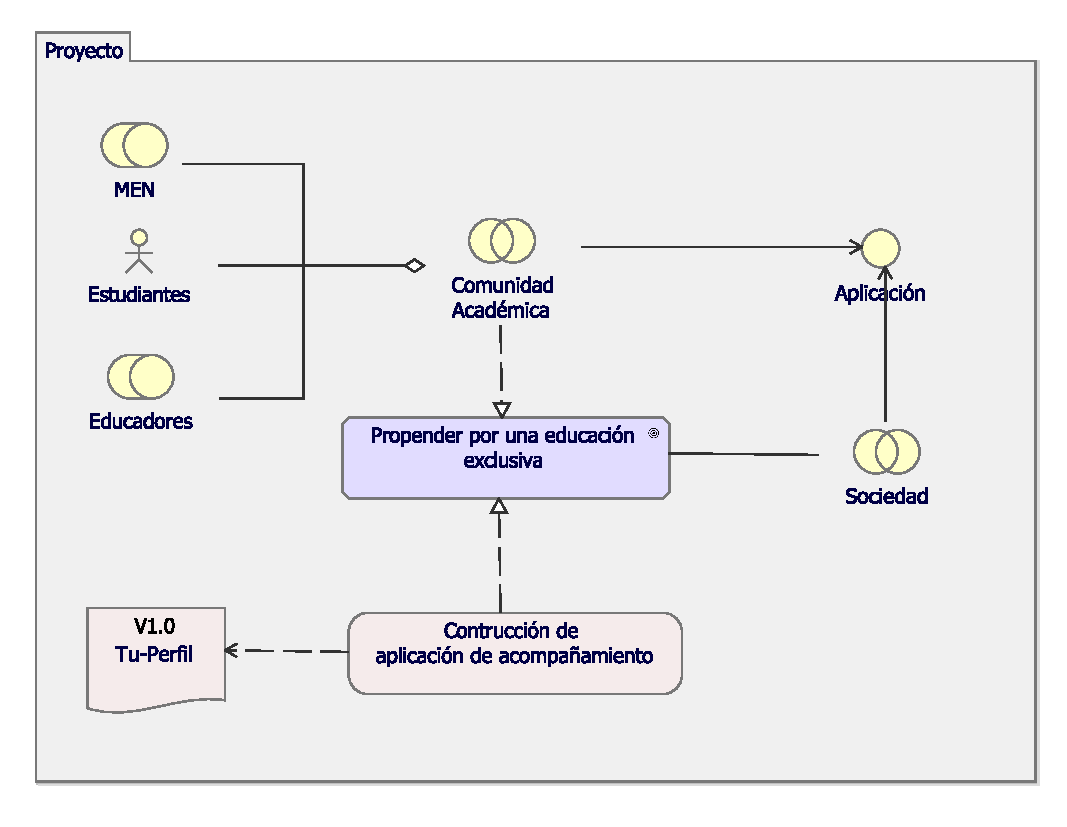
\includegraphics[width=.9\linewidth]{imgs/caso/proyecto/proyecto.pdf}
	\caption{Caso Proyecto}
\end{figure}
El objetivo que se propone por parte de la organización planteado en la capa motivacional "propender por una educación exclusiva" del cual se extiende o afecta a la comunidad académica que se compone Pone a su vez del MEN, de los estudiantes y de los educadores. Para dar alcance a este objetivo se pretende realizar la construcción de una aplicación de acompañamiento profesional, que permite el despliegue de Tu-Perfil en su versión 1.0.
\newpage
\section{Punto de Vista de Migración}
\subsection{Modelo de Migración}
\begin{figure}[h!]
	\centering
	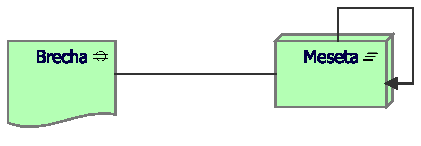
\includegraphics[width=.9\linewidth]{imgs/modelo/Migracion.pdf}
	\caption{Modelo Migración}
\end{figure}
El punto de vista de la migración implica modelos y conceptos que se pueden utilizar para especificar la transición de una arquitectura existente a una arquitectura deseada.

\subsection{Caso  de Migración}
\begin{figure}[h!]
	\centering
	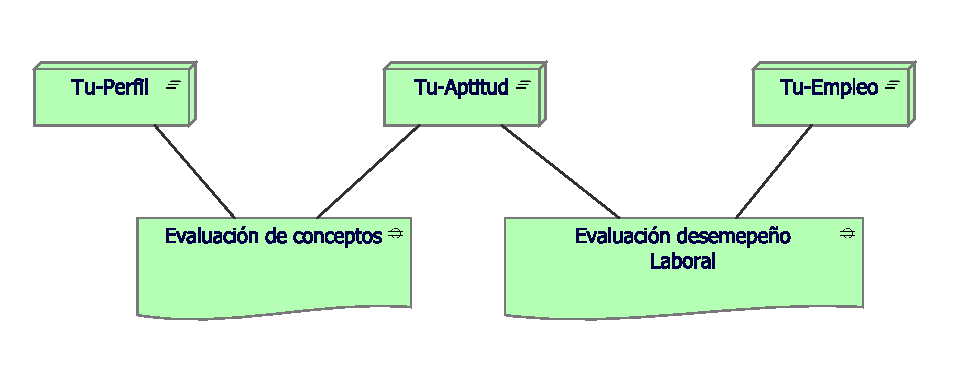
\includegraphics[width=.9\linewidth]{imgs/caso/proyecto/migracion.pdf}
	\caption{Caso Migración}
\end{figure}
En el punto visto de migración para el caso de estudio se plantea la aplicación inicial de Tu-Perfil que permitirá el perfilamiento y acompañamiento del estudiante. Como Siguiente versión se pretende implementar una aplicación (Tu-Aptitud) que evalúe de manera estricta los conceptos adquiridos durante la formación vocacional del estudiante y así lograr concebir las aptitudes más sobresalientes que ayudarán a encaminar a el estudiante a la vida profesional buscando ser apto según estas aptitudes. El siguiente paso es la construcción de una aplicación(Tu-Empleo) que evalúe el desempleo del profesión en la vida laboral, logrando establecer sus fortalezas y debilidades, además de inducir a la persona evaluada en la posibilidad no de cambiar de ambiente  laboral.
\newpage
\section{Punto de Vista de Implementación y Despliegue}

El punto de vista de la implementación y el despliegue muestra cómo se realizan una o más aplicaciones en la infraestructura. Esto comprende la asignación de las aplicaciones y componentes a los artefactos, y la asignación de la información utilizada por esas aplicaciones y componentes a la infraestructura de almacenamiento subyacente.\\

Un artefacto representa un dato que se utiliza o se produce en un proceso de desarrollo de software, o por el despliegue y funcionamiento de un sistema informático. Un artefacto representa un elemento tangible en el mundo de la informática. El artefacto es una especialización del objeto tecnológico. Se suele utilizar para modelar productos (software) como archivos de origen, ejecutables, scripts, tablas de bases de datos, mensajes, documentos, especificaciones y archivos modelo. Una instancia (copia) de un artefacto puede ser desplegada en un nodo. Un artefacto puede utilizarse para representar un componente de datos físicos que realiza un objeto de datos.\\

Un componente de aplicación o software de sistema puede ser realizado por uno o más artefactos. Un objeto de datos puede ser realizado por uno o más artefactos. Se puede asignar un nodo a un artefacto para modelar que el artefacto está desplegado en el nodo. Así pues, las dos formas típicas de utilizar el elemento del artefacto son como componente de ejecución o como fichero de datos. De hecho, éstas podrían definirse como especializaciones del elemento del artefacto.
El nombre de un artefacto debe ser preferentemente el nombre del archivo que representa; por ejemplo, orden.jar. Un artefacto puede consistir en sub artefactos.

\clearpage

\subsection{Modelo de Implementación y Despliegue}
\begin{figure}[h!]
	\centering
	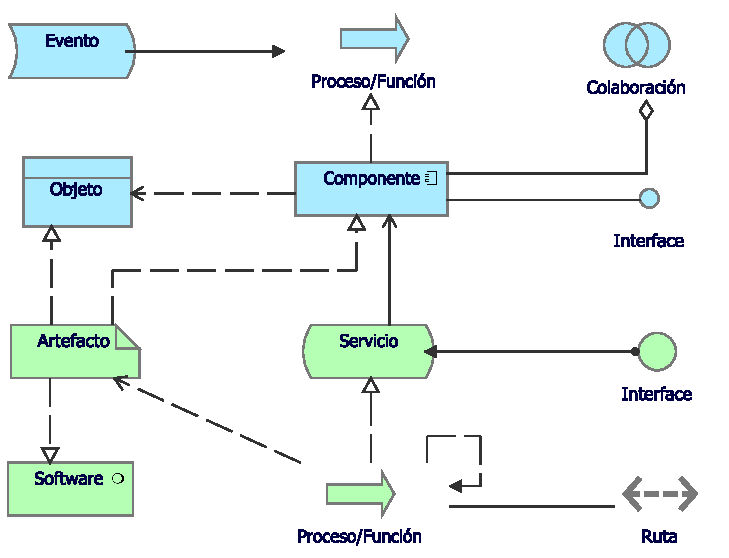
\includegraphics[width=.7\linewidth]{imgs/modelo/Implementacion}
	\caption{Modelo Implementación y Despliegue}
\end{figure}

Un objeto tecnológico modela los elementos de la estructura pasiva que son utilizados y procesados por la infraestructura. Un artefacto es una pieza física de información que se utiliza o se produce en un proceso de desarrollo de software, o por el despliegue y funcionamiento de un sistema. Es la representación, en forma de, por ejemplo, un archivo, de un objeto de datos o un componente de aplicación, y puede desplegarse en un nodo. El elemento del artefacto se ha tomado de UML. Un objeto tecnológico representa un elemento pasivo que es usado o producido por el comportamiento tecnológico. Los objetos tecnológicos representan los objetos "físicos" manipulados por la infraestructura de una empresa. Los objetos tecnológicos son elementos abstractos, es decir, no están instanciados en modelos sino que sirven como el tipo genérico de las cosas manipuladas por la Capa de Tecnología. Esto puede incluir tanto artefactos (por ejemplo, archivos) como material físico.
Se puede acceder a los objetos tecnológicos por medio del comportamiento tecnológico (funciones, procesos, interacciones, eventos y servicios). Un objeto tecnológico puede tener relaciones de asociación, especialización, agregación o composición con otros objetos tecnológicos. Un objeto tecnológico puede realizar un objeto de datos o un objeto de negocios. Puede realizarse mediante un artefacto o material (de los elementos físicos). El nombre de un objeto tecnológico debe ser preferentemente un sustantivo.

\newpage

\subsection{Caso  de Implementación y Despliegue}
\begin{figure}[h!]
	\centering
	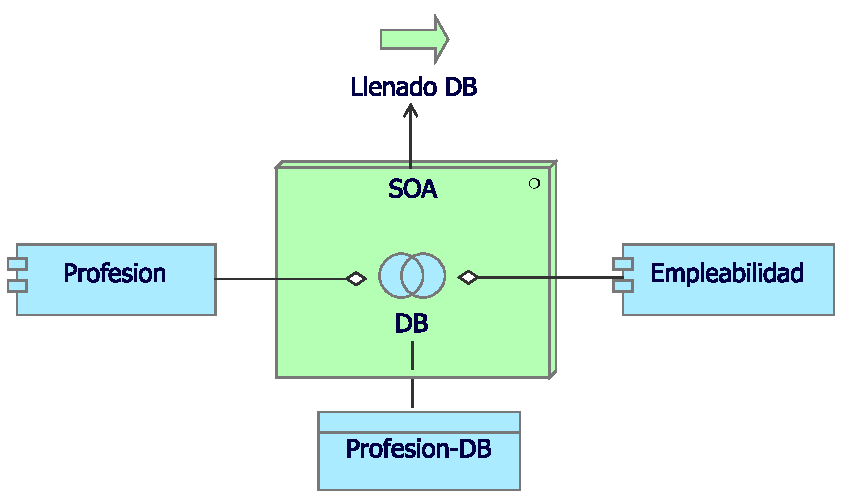
\includegraphics[width=.7\linewidth]{imgs/puntos_vista/tecnologia/despliegue.pdf}
	\caption{Caso Implementación y Despliegue}
\end{figure}

El proceso tecnológico referente al llenado de la base de datos, corresponde a una colaboración entre el componente de la aplicación Profesión y el componente externo Empleabilidad, dando como resultado la base datos de profesiones con mayor demanda en el ámbito local y fuente estadística para el posterior perfilamiento del componente Estudiante. Asimismo, se visualiza el sistema de software modelado mediante una arquitectura orientada a servicios, que facultará ese proceso tecnológico de llenado de la base de datos. En la capa de aplicación, desarrollamos una arquitectura de orquestación que permitió el modelamiento de componentes, ahora mediante la capa tecnológica y elementos tecnológicos distribuidos específicamente, además de controlar el flujo entre los componentes gracias a la arquitectura de orquestación, podemos agregar elementos externos a nuestro modelo de aplicación local.